% Compact article-format copy of the paper, for printing and reading.
% It contains no text of its own: it reads main.tex, so the two always stay in sync.
% Edit main.tex only. Compile this file (in Overleaf: Menu > Main document > main_article.tex).
\documentclass[11pt,a4paper]{article}
\usepackage[numbers,square,comma,sort&compress]{natbib}
\usepackage{authblk}
\usepackage{comment}
\usepackage{etoolbox}

% the elsarticle commands that main.tex uses, mapped to the article class
\makeatletter
\renewcommand{\documentclass}[2][]{}           % skip the \documentclass line of main.tex
\newcommand{\biboptions}[1]{}
\newcommand{\journal}[1]{}
\newenvironment{frontmatter}{}{}
\let\affiliation\affil
\newcommand{\pd@ead}{}
\newcommand{\ead}[1]{\gdef\pd@ead{#1}}
\DeclareRobustCommand{\corref}[1]{\thanks{Corresponding author. E-mail: \pd@ead}}
\newcommand{\cortext}[2][]{}
\excludecomment{highlights}
\newenvironment{keyword}{\par\medskip\noindent\textbf{Keywords:} \def\sep{; }}{\par}
\let\pd@abstract\abstract
\let\pd@endabstract\endabstract
\renewenvironment{abstract}{\maketitle\pd@abstract}{\pd@endabstract}
\makeatother

% compact page: single spacing, no line numbers, 2 cm margins
\AtBeginDocument{\newgeometry{margin=2cm}\nolinenumbers\hypersetup{hidelinks}}

\documentclass[preprint,review,12pt]{elsarticle}
\usepackage[a4paper,margin=1in]{geometry}
\let\today\relax
\makeatletter
\def\ps@pprintTitle{%
\let\@oddhead\@empty
\let\@evenhead\@empty
\def\@oddfoot{}%
\let\@evenfoot\@oddfoot}
\makeatother
%\usepackage{graphicx}
\usepackage{graphicx, subcaption}
%\usepackage{subfigure}
\usepackage{lineno}
\linenumbers
\usepackage{epstopdf}
\usepackage{color}
\usepackage{multirow}
\usepackage{textcomp,gensymb}
\usepackage{lineno}
\usepackage{xcolor}
\usepackage{physics}
\usepackage{epsfig}
\usepackage{amsmath}
\usepackage{amssymb}
\usepackage{booktabs}
\usepackage{siunitx}
\usepackage{breqn}
\biboptions{square,comma,sort&compress}
\usepackage{hyperref}
\usepackage{float}
\usepackage{adjustbox}
%\usepackage{xr-hyper}   
%\externaldocument{supplementary}
\usepackage{subfiles}
%\usepackage{credits}
\usepackage{etoolbox}
% tables and captions single-spaced; the text stays double-spaced for review
\AtBeginEnvironment{table}{\def\baselinestretch{1}}
\AtBeginEnvironment{figure}{\def\baselinestretch{1}}
\journal{}
\setlength{\textfloatsep}{12pt plus 2pt minus 2pt}  % gap between float and body text
\setlength{\abovecaptionskip}{6pt}
\setlength{\belowcaptionskip}{0pt}
\newcommand{\rev}[1]{{\color{blue}#1}}

\begin{document}
% let large floats share a page with text instead of leaving half-empty float pages
\renewcommand{\topfraction}{0.9}
\renewcommand{\bottomfraction}{0.8}
\renewcommand{\textfraction}{0.07}
\renewcommand{\floatpagefraction}{0.85}
\setlength{\emergencystretch}{3em}

\begin{frontmatter}

\title{Pydemi: A Python Package for Interpretable Charge-Density Descriptors and Materials Property Prediction} 

\author[1]{Shubham K Maurya}
\author[1]{MD Faiz Akhtar}
\author[1]{Somnath Bhowmick\corref{cor1}}
\ead{bsomnath@iitk.ac.in}
\cortext[cor1]{Corresponding author}
\affiliation[1]{Department of Materials Science and Engineering, Indian Institute of Technology Kanpur, UP 208016, India}

\begin{abstract}
The electronic charge density from a density-functional theory (DFT) calculation describes how a material is bonded, yet it is rarely used as the input of machine-learning models of material properties. Learned density representations predict properties well but are hard to interpret, while interpretable density analysis treats one structure at a time. We present pydemi, an open-source Python package that turns a VASP \texttt{CHGCAR} file into 55 interpretable descriptors of bonding, structure, and site heterogeneity. Each descriptor is stable with respect to the grid and the numerical method and is documented with its formula, units, and range. From the crystal structure alone, pydemi can also predict the density with an included ChargE3Net model; \rev{44 of the 55} descriptors of the predicted densities rank materials almost exactly as their DFT values do. \rev{pydemi computed the descriptors of 6,059 inorganic crystals without a failure, in seconds per structure.} Gradient-boosted models on the descriptors alone predict 17 elastic, thermal, energetic, electronic and optical properties, mostly with a test $R^2$ between 0.85 and 0.95. SHAP values show which descriptors drive each prediction, and ten descriptors per property are almost as good as all of them. On \rev{DFT-relaxed structures unseen by either model}, properties predicted from ML-predicted densities are nearly as accurate as those from DFT densities\rev{, so the density need not be computed}. It runs from Python, the command line, or a graphical interface.
\end{abstract}

\begin{highlights}
\item \rev{pydemi turns a VASP CHGCAR into 55 interpretable charge-density descriptors}
\item \rev{Each descriptor is stable with respect to the grid and the numerical method}
\item \rev{Descriptors alone predict 17 properties, mostly with test $R^2$ of 0.85--0.95}
\item \rev{SHAP values show which descriptors drive each property prediction}
\item \rev{ML-predicted densities give properties nearly as accurate as DFT densities}
\end{highlights}

\begin{keyword}
Electron charge density \sep Descriptors \sep Machine learning \sep Materials property prediction
\sep Interpretability \sep Python
\end{keyword}
\end{frontmatter}

\section{Introduction}
\label{sec:intro}
The electronic charge density $\rho(\mathbf{r})$ is the central quantity of
density-functional theory (DFT): it determines the ground state and all of its
properties~\cite{hohenberg1964}. It is also the most direct picture of chemical
bonding that a calculation gives. It shows where electrons accumulate between
atoms, how much charge passes from one atom to another and how localized the
electrons are. The density can also be measured by X-ray diffraction, so the
analysis methods developed for calculated densities are applied to experimental
ones as well~\cite{bader1990,abramov1997,tsirelson2002}. Every plane-wave DFT
calculation produces the density on a real-space grid, and the Materials
Project distributes such densities for a large and continuously updated set of
materials~\cite{jain2013,shen2022}. Large collections of charge densities
therefore already exist, and more are computed every day.

Over the past decade, machine learning (ML) has become a standard tool for
predicting materials properties from such databases~\cite{butler2018,schmidt2019};
we call these models property models.
How accurate a model is, and what can be learned from it, depends largely on how
each material is represented, that is, on its descriptors~\cite{ghiringhelli2015}.
Compositional featurizers compute statistics of elemental
properties~\cite{ward2016,ward2018}. Structural representations encode the
positions of the atoms, either as fixed vectors such as the Coulomb
matrix~\cite{rupp2012} and the smooth overlap of atomic
positions~\cite{bartok2013}, or as graphs from which neural networks learn their
own features~\cite{xie2018,chen2019,choudhary2021,wen2024}. All of these start
from the atoms, not from the electrons. The bonding that the density records is
learned only indirectly, from the composition and the geometry, and the most
accurate models are often the hardest to read. In materials science this
matters. {\color{red}A model whose inputs have a physical meaning can be checked against
what is known about a material, and it can point to the mechanism behind a
trend, not only to the trend itself~\cite{rudin2019}.} Methods such as SHAP
values~\cite{lundberg2020} explain the predictions of any model, but an
explanation in terms of learned features or atom embeddings is still hard to
relate to physics.

Where the density has been used as a model input, it has mostly been as a
learned representation. Three-dimensional convolutional networks read the
density on a voxel grid~\cite{kajita2017,zhao2020} or its compressed latent
representation~\cite{kumar2026}, and persistent homology reduces it to Betti
curves over density thresholds~\cite{szymanski2025}. These representations
predict properties well, which shows that the density carries the information
a property model needs. Their features, however, have no individual physical
meaning. Such models therefore share the difficulty of the graph networks: they
show how well a property can be predicted, but not which feature of the bonding
sets it. They also have to process the full grid of every structure, which makes
training and prediction costly.

{\color{red}Density analysis itself, on the other hand, has a long tradition of
interpretable quantities. The quantum theory of atoms in molecules divides the
density into atomic basins and describes each bond by the critical point between
two atoms~\cite{bader1990}. Hirshfeld partitioning shares the density between
atoms in proportion to the densities of the free atoms~\cite{hirshfeld1977}.}
The electron localization function~\cite{becke1990} shows where electrons are
paired, and the non-covalent interaction index~\cite{johnson2010} shows where
weak interactions occur. Each of these quantities has a clear meaning, and
together they describe ionic, covalent and metallic bonding in terms that
chemists and physicists share. They are computed by programs such as
critic2~\cite{oterodelaroza2014} and the Bader code~\cite{henkelman2006}, which
are built to analyse one structure in depth. Their output is a list whose length
varies from structure to structure, with one entry per atom, bond or critical
point, and not a fixed-length vector that a property model can take. The
numerical choices behind the output, such as the grid, the interpolation and the
integration method, are left to the user. Applying these programs to thousands
of structures, in a way that gives the same answer for the same material, is
not what they were designed for.

Turning the density into fixed-length descriptors for many structures raises
three problems. The first is the input and its numerics. {\color{red}The file that every
VASP calculation writes, the \texttt{CHGCAR}, holds the density on a grid but
not the wavefunctions, so it does not support every quantity of density
analysis. The electron localization function and the energy densities, for
example, need the kinetic energy density, which the density alone gives only
approximately~\cite{abramov1997,tsirelson2002}.} A quantity computed on a grid
can also depend on the grid spacing, on the numerical derivatives and on the way
the cell is written down as much as on the material, and a descriptor of this
kind adds noise that no model can remove. The second problem is cost. A
descriptor that needs a DFT density needs a DFT calculation, which limits it to
materials that have already been computed. Models that predict the density from
the atomic structure~\cite{chandrasekaran2019,grisafi2019,jorgensen2022,koker2024}
remove this limit in principle, provided the descriptors survive the error of
the prediction. {\color{red}This is not guaranteed: descriptors built from derivatives of
the density, such as the curvature of a bond, enlarge small errors of the
density. The third problem is the question that motivates the descriptors in the
first place: how much of a material's properties they capture, and which of
them carry the information.} A few chosen examples cannot answer it. It has to be
answered on a large, well-defined dataset and for many properties at once.

Here we describe pydemi, a Python package built around these three problems.
(i) It reads one file, the VASP \texttt{CHGCAR}, and computes 55 descriptors
{\color{red}that are defined on it and whose values are set by the material, not by the
grid or the numerical method (for a given choice of PAW potentials)} (Sections~\ref{sec:design}
and~\ref{sec:descriptors}). The descriptors describe how the charge is
distributed around each nucleus and between the atoms, the shape of the density
over the whole cell, and how much the atoms of a crystal differ from one
another. Each has a short physical definition, and each is checked by automated
tests against densities with known answers and against different descriptions of
the same crystal. (ii) It includes a density
model, so that the same descriptors are obtained from a crystal structure alone,
and we measure which descriptors transfer from DFT to predicted densities
(Section~\ref{sec:ml}). (iii) We train property models on the descriptors alone
for 17 properties of a large DFT dataset, compare them with the models reported
earlier for the same structures, and identify the descriptors that carry the
information (Section~\ref{sec:properties}). The package is used as a Python
library, a command-line tool or a graphical interface that runs locally
(Section~\ref{sec:software}); the code, the tests and the scripts that train the
property models are released under the MIT license.

% ==========================================================================
\section{Methodology}
\label{sec:design}

Pydemi needs one file, the VASP \texttt{CHGCAR} (or \texttt{CHG}), plain or
compressed. The structure is read from its header and the total density from
the first data block, which is divided by the cell volume to give $\rho$ in
e\,\AA$^{-3}$. Spin-polarized and non-collinear files are accepted, and their
magnetization blocks are ignored. No other VASP file (\texttt{POTCAR},
\texttt{OUTCAR}, \texttt{AECCAR}, \texttt{ELFCAR}, \texttt{LOCPOT}) is needed,
and the atomic radii used for the shells and the partitions are tabulated in the
package. This is a deliberate choice: every VASP run writes a \texttt{CHGCAR}, so
any collection of calculations can be \rev{processed} without going back to the
original runs, and no descriptor depends on a file that some structures have and
others do not. The density can also come from a crystal structure through the
included ChargE3Net model (Section~\ref{sec:ml}). Both routes give the same
density object (Fig.~\ref{fig:architecture}), an instance of the
\texttt{VolumetricData} class of the package, which holds the structure, the density grid and a note of where the density came from; this note
is written into the metadata of every output row.

\begin{figure}[!t]
\centering
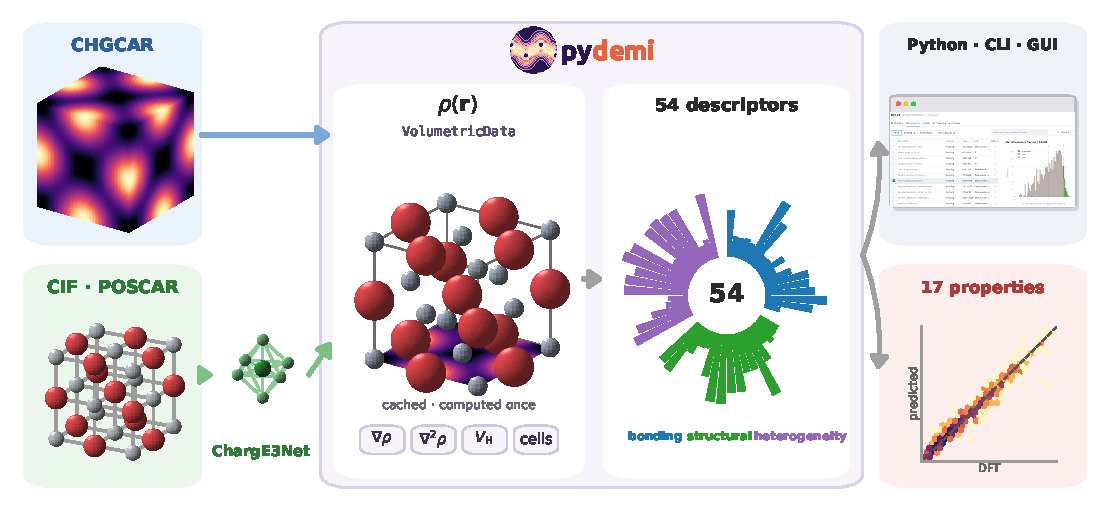
\includegraphics[width=\textwidth]{figures/fig_architecture.pdf}
\caption{Architecture of pydemi, drawn for MgO. A DFT \texttt{CHGCAR} (left, top) and a crystal structure (CIF, POSCAR, or any format ASE reads) whose density is predicted by the included ChargE3Net model (left, bottom) give the same density grid $\rho(\mathbf{r})$, shown as the $1.5$~e\,\AA$^{-3}$ isosurface around O, the Mg atoms, and the density on one face of the cell. Inside pydemi (center box), the grid is held in the density object; the derived fields (gradient, Laplacian, Hartree potential $V_H$) and the atomic cells of the geometry pass are computed once per structure and cached on the structure; the descriptors then reduce them to single numbers. The radial bars show the percentiles for each MgO descriptor within the dataset, grouped by domain. The descriptors are used from Python, the command line, or the graphical interface (right, top: a screenshot, Fig.~\ref{fig:gui}), and the property models of Section~\ref{sec:properties} take them as input (right, bottom: test predictions of the bulk modulus).}
\label{fig:architecture}
\end{figure}

From the density grid, pydemi first computes the fields and the geometry that
the descriptors need, and it computes each of them only once per structure. A
derived quantity, such as the gradient, the Hartree potential or the map from
each grid point to its nearest atom, is stored on the density object
the first time a descriptor asks for it, and every later descriptor that
needs it reuses the stored copy. The settings it was computed with (for example
the derivative method or the shell radii) are stored with it, so a structure
\rev{processed} again with other settings gets new fields and never stale ones.

{\color{red}% unclear, to rewrite
VASP cells are often not orthogonal, so the derivatives are taken along the axes
of the grid and then converted to Cartesian ones. For the Laplacian this
conversion has cross terms between the grid axes,
\[
\nabla^2 f=\sum_{a,b}G_{ab}\,\frac{\partial^2 f}{\partial u_a\,\partial u_b},
\]
where $u_a$ are the fractional coordinates and $G=BB^{\mathsf T}$ is built from
the reciprocal lattice vectors (the rows of $B$). The cross terms vanish only
for orthogonal axes; leaving them out, a common shortcut, makes the Laplacian of
a triclinic test cell more than 5\% wrong. By default the derivatives are
computed in Fourier space, where each one becomes a multiplication. A plane-wave
density is a finite Fourier series, so this is exact up to round-off; finite
differences are available as an alternative and are compared in
Section~\ref{sec:descriptors}. The Hartree potential of the electrons comes from
the same Fourier coefficients by solving Poisson's equation, and since its
average is undefined for a periodic system, it is measured from its cell
average.}

Many descriptors need to know, for every grid point, which nucleus is nearest,
how far away it is and in which direction. These are computed once with a
$k$-d tree over the atoms and their periodic images. In strongly sheared cells
the nearest image can lie beyond the usual $3\times3\times3$ block of cells, so
the search is widened until it is guaranteed to contain it. Some grid points
lie at exactly the same distance from two or more nuclei, which is common when
atoms sit on high-symmetry grid points. Such a point is given to one of these
nuclei by a rule that {\color{red}uses only their positions relative to the point, not the
order in which the atoms are listed in the file. The point then goes to the
equivalent atom in a cell, in its supercell and in a translated or rotated copy,
so the descriptors do not change between these cells
(Section~\ref{sec:descriptors}).} The distance to the nearest nucleus also
divides the cell into three regions: the core (within 0.8\,\AA{} of a
nucleus), the bond shell (0.8 to 1.5\,\AA) and the interstitial region (beyond
1.5\,\AA). These boundaries can instead be set for each atom as multiples of
its covalent radius. \rev{All results in this work, including the property
models, use the fixed boundaries. They put every material on the same length
scale, so that the larger cores of heavy atoms show up in the descriptors
instead of being scaled away; \texttt{pydemi sweep} shows how the descriptors
change when the boundaries are moved (Section~\ref{sec:software}).} {\color{red}The descriptors
that are resolved per atom need to know which grid points belong to which atom,
and three ways of dividing the cell are offered: nearest-atom (Voronoi) cells,
the default; a power diagram, which gives larger atoms larger cells; and the
fuzzy cells of Becke~\cite{becke1988}, which share each point between
neighbouring atoms with smooth weights. All three return weights that sum to one
at every point, so every per-atom descriptor works with any of them unchanged.}

Each descriptor is a short Python function that takes the
density object and returns one number. It is added to a single list of all
descriptors (the registry) together with a record that describes it: its name, its domain
(bonding, structural or heterogeneity), the cached quantities it needs, its
units, the range of values it can take, its formula and references, and the
cases in which it is undefined, each with the constant returned instead. A
uniform density, for instance, has no gradient, so the non-radial
gradient share is zero divided by zero; the descriptor returns 0 and is flagged, {\color{red}and
the output then carries a companion flag column set to 1}, so a user can find and
exclude such values. No descriptor returns a bare NaN, with one documented
exception: {\color{red}the within-element variances of Table~\ref{tab:families2}, when no
element has two or more atoms in the cell (for example the two-atom cell of
MgO), so there are no atoms of the same element to compare.}

This list is the source from which everything else is built. The
feature vector always has the descriptors in the order in which they were
added, so its columns never change between runs. The catalogue of names,
units, ranges, formulas and undefined cases is read from it, and so are the
invariance tests of Section~\ref{sec:descriptors}, so a descriptor added later is
tested without writing a new test. A quantity that grows with the size of the cell, such as a total
charge or a number of density maxima, is refused when it is added; it has to be divided by the volume, the number of atoms or the total charge
first, and the supercell test then checks that the result really does not
change with the cell size.

Throughout this work, pydemi is applied to the charge densities of 6,059
inorganic crystals of 87 elements from our earlier study~\cite{kumar2026},
computed with VASP~\cite{kresse1996} and the PBE functional~\cite{perdew1996}
for structures taken from the Materials Project; the structures and the DFT
settings are described there. \rev{In brief, the calculations used PAW
potentials~\cite{blochl1994,kresse1999}, a plane-wave cutoff of 500\,eV and a
$k$-point spacing of 0.1\,\AA$^{-1}$, and each density comes from a final
calculation with the tetrahedron method (Section~S7 of the Supporting
Information). Each element has one PAW dataset throughout the set. For 41 of the 87
elements it differs from the one in the input set of the Materials Project,
mostly by having
fewer semicore electrons in the valence (for example Ti instead of Ti\_pv) or,
for the lanthanides, by keeping the $f$ electrons in the valence; Table~S9 of
the Supporting Information lists them.} The set contains elemental solids, intermetallic
compounds and compounds of metals with non-metals (borides, carbides, hydrides,
pnictides, chalcogenides, oxides and halides), so metallic, covalent and ionic
bonding are all well represented. The number of structures in each class is
given in Section~S7 of the Supporting Information.

% ==========================================================================
\section{The descriptors}
\label{sec:descriptors}

Tables~\ref{tab:families} and~\ref{tab:families2} give each descriptor a
descriptive name, its name in the package and a one-line definition; the full
definitions, units, ranges, references and fallback values are given in
Section~S1 of the Supporting Information and in the reference document of the
package. In what follows $k$ runs over the grid points,
$i(k)$ is the nearest nucleus of grid point $k$, $r_k$ its distance and
$\hat{\mathbf u}_k$ the unit vector from that nucleus to the grid point.

\begin{table}[!tp]
\centering
\caption{The 18 bonding descriptors of pydemi, with a descriptive name and
the name used in the package. Core, bond shell and interstitial region
as defined in Section~\ref{sec:design}. The signed NCI density is given in
atomic units, as is usual for this quantity. Formulas, ranges, references and fallback values:
Supporting Information, Section~S1.}
\label{tab:families}
\footnotesize
\setlength{\tabcolsep}{4pt}
\begin{adjustbox}{max width=\textwidth}
\begin{tabular}{@{}>{\raggedright\arraybackslash}p{3.7cm}l>{\raggedright\arraybackslash}p{5.4cm}l@{}}
\toprule
Name & Name in pydemi & Definition & Units \\
\midrule
Mean charge distance & \texttt{m1} & mean distance of the charge from its nearest nucleus & \AA \\
Mean squared charge distance & \texttt{m2} & mean squared distance of the charge from its nearest nucleus & \AA$^2$ \\
Charge-distance variance & \texttt{sigma\_r2} & variance of the distance of the charge from its nearest nucleus & \AA$^2$ \\
Core charge fraction & \texttt{f\_core} & fraction of the charge in the core & -- \\
Bond-shell charge fraction & \texttt{f\_bond} & fraction of the charge in the bond shell & -- \\
Interstitial charge fraction & \texttt{f\_int} & fraction of the charge in the interstitial region & -- \\
Non-radial gradient share & \texttt{zeta} & non-radial share of the density gradient (0 for spherical atoms) & -- \\
Negative-Laplacian volume fraction & \texttt{lnf} & volume fraction with negative Laplacian (charge concentrated) & -- \\
Negative-Laplacian charge fraction & \texttt{lnf\_charge\_weighted} & fraction of the charge where the Laplacian is negative & -- \\
Valence Laplacian concentration & \texttt{lap\_concentration\_valence} & share of the absolute Laplacian outside the cores where it is negative & -- \\
Mean bond ellipticity & \texttt{ellip\_bond\_bounded\_avg} & mean bounded bond ellipticity in the bond shell: 0 cylindrical, 1 flat & -- \\
Non-covalent interaction (NCI) volume fraction & \texttt{f\_NCI} & volume fraction of the NCI region (low density, low gradient) & -- \\
Attractive NCI fraction & \texttt{NCI\_attractive} & fraction of the NCI region that is attractive & -- \\
Signed NCI density & \texttt{sign\_lambda2\_rho\_mean} & signed mean density of the NCI region (negative where attractive) & e\,bohr$^{-3}$ \\
Site potential spread & \texttt{V\_spread} & standard deviation of the electronic Hartree potential at the atoms & eV \\
Interstitial potential minimum & \texttt{V\_int\_min} & lowest electronic Hartree potential in the interstitial region & eV \\
Mean bond-midpoint density & \texttt{rho\_mid\_mean} & mean density at the bond midpoints & e\,\AA$^{-3}$ \\
Bond-midpoint density spread & \texttt{rho\_mid\_std} & standard deviation of the density at the bond midpoints & e\,\AA$^{-3}$ \\
\bottomrule
\end{tabular}
\end{adjustbox}
\end{table}

\begin{table}[!tp]
\centering
\caption{The 19 structural and 18 site-heterogeneity descriptors of pydemi,
as in Table~\ref{tab:families}. Density shape: the density divided by the
number of electrons. The Fisher information is given in atomic units.}
\label{tab:families2}
\footnotesize
\setlength{\tabcolsep}{4pt}
\begin{adjustbox}{max width=\textwidth}
\begin{tabular}{@{}>{\raggedright\arraybackslash}p{3.7cm}l>{\raggedright\arraybackslash}p{5.4cm}l@{}}
\toprule
Name & Name in pydemi & Definition & Units \\
\midrule
\multicolumn{4}{@{}l}{\emph{Structural (19)}} \\
Percolation densities & \texttt{rho\_perc\_a}, \texttt{\_b}, \texttt{\_c} & highest density level still connected across the cell along $\mathbf a$, $\mathbf b$, $\mathbf c$ & e\,\AA$^{-3}$ \\
Percolation anisotropy & \texttt{perc\_anisotropy} & spread of the three percolation levels relative to their mean & -- \\
Density maxima per volume & \texttt{n\_max} & number of local maxima of the density per volume & \AA$^{-3}$ \\
Density minima per volume & \texttt{n\_min} & number of local minima of the density per volume & \AA$^{-3}$ \\
Non-nuclear maxima per volume & \texttt{n\_NNM} & density maxima farther than 0.8\,\AA{} from every nucleus, per volume & \AA$^{-3}$ \\
Non-nuclear-maximum charge & \texttt{Q\_NNM} & fraction of the charge in the basins of these non-nuclear maxima & -- \\
Minimum density & \texttt{rho\_min} & lowest density in the cell & e\,\AA$^{-3}$ \\
Relative minimum density & \texttt{rho\_min\_ratio} & lowest density divided by the mean density & -- \\
Mean interstitial density & \texttt{rho\_int\_mean} & mean density in the interstitial region & e\,\AA$^{-3}$ \\
Gradient-direction eigenvalues & \texttt{T\_eigenvalues\_t1}, \texttt{\_t2}, \texttt{\_t3} & eigenvalues of the tensor of gradient directions; all $\tfrac13$ if isotropic & -- \\
Gradient fractional anisotropy & \texttt{charge\_FA} & fractional anisotropy of that tensor: 0 isotropic, 1 along one axis & -- \\
Shannon entropy & \texttt{shannon\_entropy} & Shannon entropy of the density shape; 0 for a uniform density & -- \\
Disequilibrium & \texttt{disequilibrium} & mean squared density shape; 1 for a uniform density & -- \\
LMC complexity & \texttt{LMC\_complexity} & statistical complexity of L\'opez-Ruiz, Mancini and Calbet~\cite{lopezruiz1995} & -- \\
Fisher information & \texttt{fisher\_information} & Fisher information of the density shape; large for steep changes & bohr$^{-2}$ \\
\addlinespace
\multicolumn{4}{@{}l}{\emph{Site heterogeneity (18): \texttt{X} = \texttt{m1}, \texttt{f\_bond} or \texttt{zeta} of each atom, from its own atomic region}} \\
Site spread of \texttt{X} & \texttt{X\_site\_std} & standard deviation of \texttt{X} over the atoms & as \texttt{X} \\
Site range of \texttt{X} & \texttt{X\_site\_range} & largest minus smallest \texttt{X} over the atoms & as \texttt{X} \\
Site maximum, minimum of \texttt{X} & \texttt{X\_site\_max}, \texttt{\_min} & largest and smallest \texttt{X} over the atoms & as \texttt{X} \\
Within-element variance of \texttt{X} & \texttt{X\_within\_element\_var} & part of the variance of \texttt{X} from differences within each element & \texttt{X}$^2$ \\
Between-element variance of \texttt{X} & \texttt{X\_between\_element\_var} & part of the variance of \texttt{X} from differences between elements & \texttt{X}$^2$ \\
\bottomrule
\end{tabular}
\end{adjustbox}
\end{table}

The bonding descriptors ask how the charge is arranged around the atoms and in
the bonds. The radial moments $m_n=\sum_k\rho_k r_k^n/\sum_k\rho_k$ and the shell
fractions describe how far the charge sits from its nearest nucleus; a large
interstitial fraction points to delocalized charge between the atoms. The
non-radial gradient share
\begin{equation}
\zeta = 1-\frac{\sum_k|\nabla\rho_k\cdot\hat{\mathbf u}_k|}{\sum_k|\nabla\rho_k|}
\end{equation}
vanishes for spherical, non-overlapping atoms and grows as charge is pulled off
the radial direction. The Laplacian descriptors locate where charge is
concentrated ($\nabla^2\rho<0$). The share of $|\nabla^2\rho|$ that lies where
$\nabla^2\rho<0$ is computed only outside the cores: over {\color{red}the whole cell
$\nabla^2\rho$ integrates to zero, so this share would be $\tfrac12$ for every
crystal.} {\color{red}The bounded ellipticity distinguishes
cylindrical from flattened charge in the bond shell,} and the non-covalent interaction (NCI) descriptors
pick out the low-density, low-gradient regions of weak
interactions~\cite{johnson2010}. The structural descriptors treat the density of
the whole cell. \rev{They measure} how well {\color{red}it connects (percolation levels, detected by a
union--find over periodic images)}, its maxima, minima and non-nuclear maxima,
its lowest density, its directionality and its information content. {\color{red}The heterogeneity descriptors turn per-atom values of $m_1$, $f_{bond}$ and $\zeta$ into
statistics over the atoms, including the decomposition
$\text{Var}_iX=\sum_e x_e\text{Var}_{i\in e}X+\sum_e x_e(\bar X_e-\bar X)^2$
into within- and between-element parts, where $x_e$ is the fraction of the atoms
that belong to element $e$; the decomposition is exact, as in a one-way analysis of variance.}
Every descriptor is invariant under supercell expansion, rotation and
translation of the crystal by whole grid steps, {\color{red}except the within-element
variances of a cell in which every element has a single atom: they are undefined
(Section~\ref{sec:design}), while a supercell of the same crystal gives zero.
This affects 421 of the 6,059 materials of our dataset, and the property models
of Section~\ref{sec:properties} treat these values as missing}.

A descriptor should describe the material, not the way it was computed. Three
things in a pydemi calculation are not set by the material. The first is the
density grid: VASP chooses it from the plane-wave cutoff, so two calculations
of the same compound can give grids of different fineness. The second is the
way the derivatives of the density, which several descriptors need, are
computed. The third is the division of the cell into atomic regions, which
the site descriptors use. If a descriptor changed noticeably when the grid or
the derivative method changed, the
same material could get different values, and a model trained on the
descriptor would learn this noise instead of the material.

We therefore tested the first two on structures of our dataset. For the grid, we recomputed the descriptors on a
coarser grid with about half as many points, as a calculation with a lower
cutoff would give. For the derivatives, we replaced the default method, which
takes exact derivatives from the Fourier transform of the density, by the
simpler finite differences.

Most descriptors are insensitive to both choices. On the coarser grid, the
median change is below 1\% for 46 of the 55. Most of the few that change more
have values close to zero for many materials, {\color{red}for example the percolation
anisotropy of a cubic crystal, or the spread between atoms of an element that are all
equivalent by symmetry. For such values, a tiny absolute change is a large
percentage. The number of non-nuclear maxima changes for a different reason: a
coarser grid can miss small maxima. Fourth-order finite differences give the
same values as the default method to better than 1\%, which confirms that the
default is accurate. Second-order ones change some descriptors by up to
16\%, so pydemi does not use them by default.}

{\color{red}The PAW potentials are a further choice that the material does not set. A
\texttt{CHGCAR} holds the valence pseudo-density, so a potential that treats more
electrons as valence, such as the semicore $3p$ electrons of Ti\_pv, adds charge
near the nuclei and changes the descriptors that measure it. To see how large this
effect is, we computed the descriptors from the densities that the Materials
Project distributes for 80 of our test materials. The Materials Project computed
them with its own structures, cutoffs and $k$-points. For the 40 materials whose
elements all have the same potentials as in our dataset, the densities agree
well: 44 of the 55 descriptors still rank the materials in the same order
($\rho_s\geq0.95$), and the median change of a descriptor is about 1.5\%. The
property models score almost the same from both densities. For the 40 materials
with at least one other potential, the median change is about 20\%. Only four
descriptors keep the ranking: the mean interstitial density, the mean and spread
of the bond-midpoint density and one percolation level. The bulk modulus, which
rests mainly on the interstitial density, is predicted as well as before. The
scores for the sound velocities, the Debye temperature and the energies, however,
drop by 0.15 to 0.25. The descriptors are therefore set by the material for a
given set of potentials. The property models of pydemi should be used with
densities computed with the potentials of our dataset (Table~S9 of the
Supporting Information). A
\texttt{CHGCAR} does not record its potentials, so pydemi cannot check this.
Section~S8 of the Supporting Information gives the comparison for every
descriptor and property.}

{\color{red}The site descriptors also depend on the division into atomic regions. This is
not an error: a different division describes different regions, so pydemi
treats it as a setting and records it with every result. Section~S2 of the
Supporting Information gives the change of every descriptor for every choice,
including the division into atomic regions. It also explains which quantities
of density analysis pydemi does not offer because a \texttt{CHGCAR} cannot
support them reliably. An example is the electron localization function, which needs
more than the density~\cite{abramov1997,tsirelson2002}. Finally, it explains what the PAW
pseudo-density~\cite{blochl1994,kresse1999} stored in a \texttt{CHGCAR} means
for the descriptors.}

A descriptor must also be computed correctly. pydemi is therefore checked by
automated tests that run every time the code changes. Each test computes
something with pydemi and compares it with an answer that is known
independently. Two kinds of tests check the descriptors.

The first kind checks that each descriptor computes what it claims. These tests
run pydemi on artificial densities for which the right answer is known exactly from a
formula. Two model atoms are used: smooth Gaussian atoms, and Slater-type atoms, which
have the sharp peak at the nucleus that real atoms have. For example, the
average distance of the charge from its nucleus must equal the textbook value
for a Slater atom, and the derivatives and the electrostatic potential that
pydemi computes must equal the exact ones. Other tests use rules that hold for
any density: the charge fractions of the core, bond and interstitial regions
must add up to one, and the parts of a variance must add up to the whole.
Where no formula exists, pydemi is compared with a slow but simple calculation,
such as finding the nearest atom by searching all neighbouring cells.

The second kind checks that a descriptor stays the same when the crystal is
described differently. The same material can be written down in many ways, and
a descriptor must not depend on the choice. For a low-symmetry test crystal,
every descriptor is computed four times: for the original cell, for a cell
eight times larger, for the cell with its origin moved by a whole number of grid steps, and for the cell
rotated in space. All four must give the same value. These symmetry tests are
generated automatically from the list of descriptors, so a descriptor added in
the future is checked without writing a new test.

No two computer calculations agree to the last digit, so each test allows a
small difference, chosen from what can cause it. Where only rounding can cause
it, the allowed difference is one part in a billion or less\rev{. It is} one part in a
million for the symmetry tests, whose sums run over the grid in a different
order\rev{. Where} the grid
cannot represent a sharp atomic peak exactly, it is larger and set from the
known size of this grid error\rev{. These} tests also check that the error shrinks
when the grid is refined. Each test, its reference and its allowed difference are listed in Section~S6 of
the Supporting Information.

% ==========================================================================
\section{Descriptors from a predicted density}
\label{sec:ml}

pydemi includes ChargE3Net~\cite{koker2024}, a neural network that predicts the
electron density of a crystal from its atomic structure alone. Its authors
released the network together with weights trained on the charge densities of
the Materials Project~\cite{shen2022}. These weights cannot be used for our
dataset as they are: for several elements the Materials Project used different
PAW potentials, and hence a different number of valence electrons, so its
predictions differ strongly from our DFT densities. We therefore started from
the released weights and continued the training on the densities of our dataset
(fine-tuning), with 5,152 structures for training, 302 for validation and 605
for testing. \rev{This} gave a lower error than training the same network from
scratch on our data. The fine-tuned model is the one included in pydemi, so its
predictions stand for a \texttt{CHGCAR} computed with the settings of our
dataset~\cite{kumar2026}. pydemi places it on the grid that VASP would use
for these settings, scales it to the right number of valence electrons and
records how it was obtained. \rev{It then} computes every descriptor from it
exactly as from a \texttt{CHGCAR}. The model covers the 87 elements of the
dataset and refuses structures with other elements. The network code in pydemi
is a copy of the original one that runs without its training framework, and it
gives the same predictions. \rev{Its} cost grows with
the number of atoms and grid points, and a GPU is used when one is available.
Technical details are given in Section~S2 of the Supporting Information.

\begin{figure}[htbp]
\centering
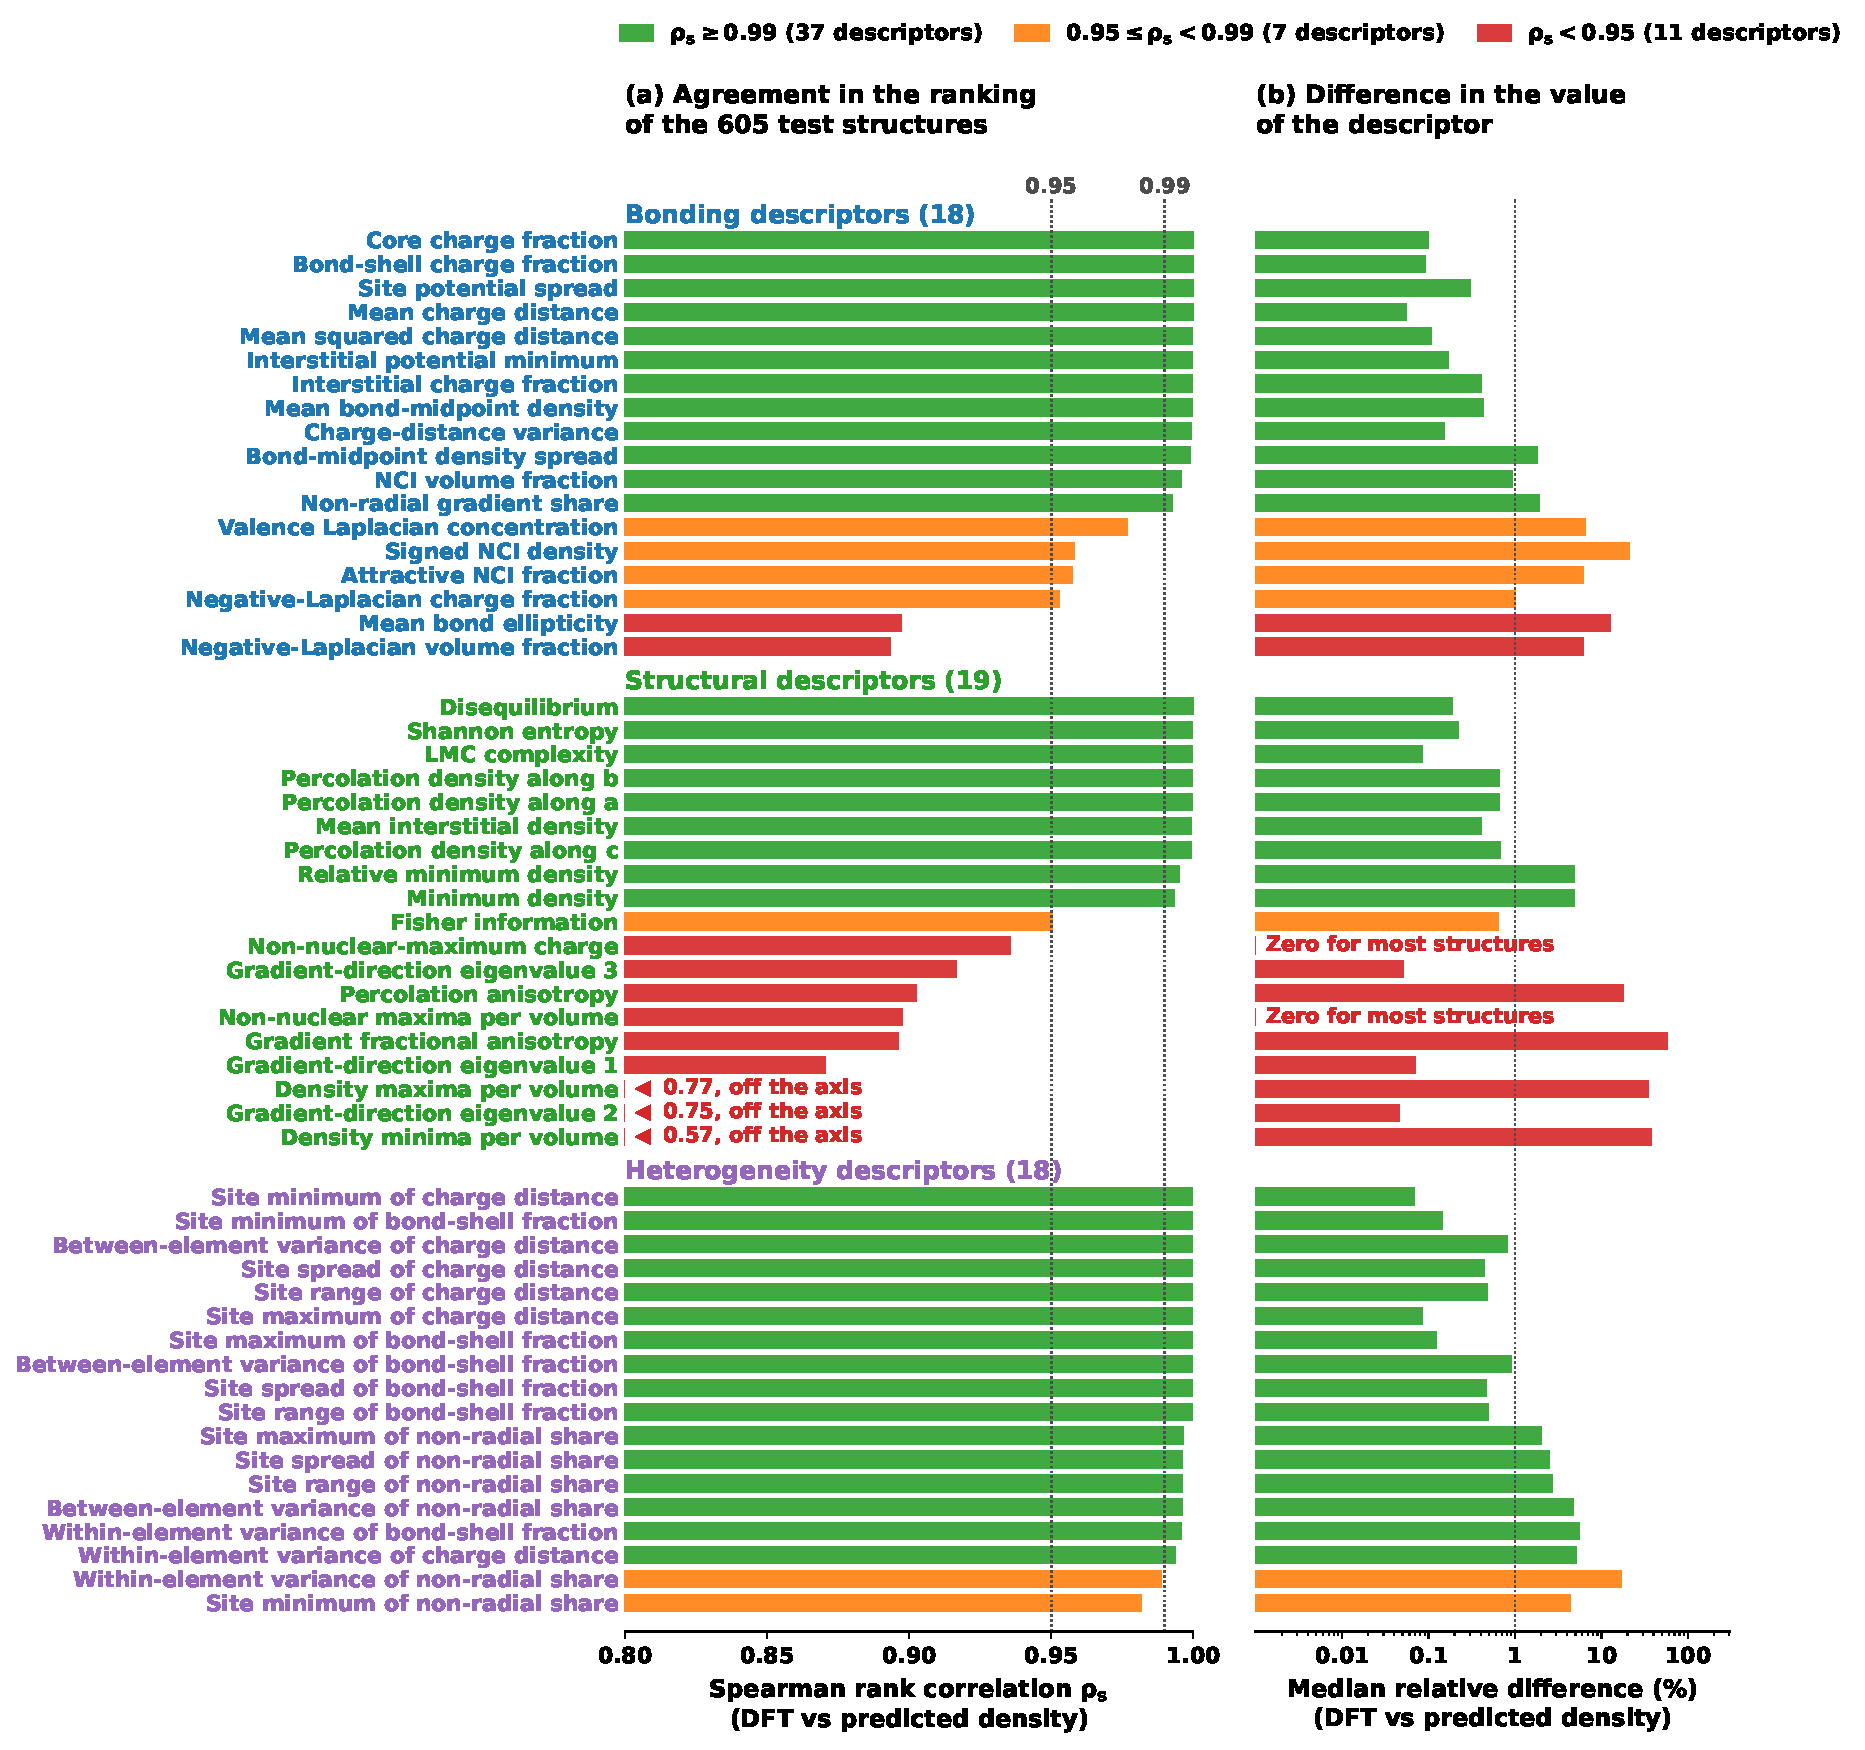
\includegraphics[width=\textwidth]{figures/fig_ml.pdf}
\caption{Descriptors from predicted densities: the descriptors of the test
structures of the density model, computed from the DFT and from the ChargE3Net
density, grouped by domain. (a) Spearman rank correlation $\rho_s$ between the two
sets of values (axis from 0.8 to 1; the three descriptors below 0.8 are marked
with their value; dotted lines at 0.95 and 0.99). (b) Median relative error
$|a-b|/\max(|a|,|b|)$ over the structures (logarithmic axis; 0 where both values
are zero for most structures, as for the non-nuclear maxima). Colours: green
$\rho_s\geq0.99$, orange $0.95\leq\rho_s<0.99$, red $\rho_s<0.95$. Parity plots of every
descriptor are given in Figs.~S2 and S3 of the Supporting Information.}
\label{fig:ml}
\end{figure}

The predicted densities are close to the DFT ones\rev{. The} absolute difference summed over the grid is about 0.6\% of
the total charge (median over the test structures)\rev{. It is} somewhat larger for crystals with lanthanides or actinides. The question for
pydemi is whether such small differences change the descriptors. A descriptor
helps a property model when it puts materials in the right order. \rev{We
therefore} measured, for each descriptor, whether its values from the DFT and from the
predicted densities rank the test materials in the same order (Spearman
rank correlation $\rho_s$, which is 1 for the same order). For 44 of the 55
descriptors, $\rho_s$ is at least 0.95, and for 37
of them at least 0.99 (Fig.~\ref{fig:ml}a), and most of them change by
less than 1\%. They include all 18 heterogeneity descriptors, 16
of the 18 bonding descriptors, and the percolation levels, the lowest and
the mean interstitial density, and the information measures. The other 11 fall into three groups, each with a
clear reason. The counts of maxima and minima of the density change because the
prediction adds or removes tiny bumps in flat regions far from the atoms,
without changing the density noticeably. \rev{The} number and charge of non-nuclear
maxima are zero in both densities for most structures, so their ranking is
decided by a few materials. The bounded bond ellipticity and the volume
fraction of negative Laplacian use second derivatives of the density in
low-density regions, and derivatives magnify the small errors of the
prediction. \rev{The last group are five anisotropy measures: the three eigenvalues and the
fractional anisotropy of the tensor of gradient directions, and the percolation
anisotropy. They are predicted accurately, but many materials share almost the
same value (every cubic crystal, for instance, is isotropic), so tiny
differences reorder them. Several of these values are close to zero, so their
relative error in Fig.~\ref{fig:ml}b looks large although the absolute
difference is small.} When
the density is predicted, the 44 can therefore be used as they are, and the
other 11 with care. \rev{For these 11, the value from a predicted density
should not be used to rank or compare individual materials; where a DFT
density exists, its value should be used instead. The property models still use
all 55, and Section~\ref{sec:properties} measures what this costs.} The Compare view of the graphical
interface (Section~\ref{sec:software}) shows, for a given \texttt{CHGCAR}, the
descriptors of the DFT and of the predicted density side by side, together with
the transfer of each descriptor. Only five of the test structures have a
median error over the 44 descriptors above 5\% (Supporting Information, Fig.~S4). Like the
DFT path, which uses the total density of a \texttt{CHGCAR}, the model predicts
the total density only, so neither path provides magnetic descriptors.

% ==========================================================================
\section{Property prediction}
\label{sec:properties}

\subsection{Data and protocol}
We used the descriptors to predict 17 properties of the materials of the dataset.
\rev{All 17 were downloaded from the Materials Project~\cite{jain2013}
(database version 2026.04.13). They are the bulk, shear and Young's moduli;} the
elastic constants $C_{11}$, $C_{12}$ and $C_{44}$~\cite{dejong2015}; the Debye
temperature, the \rev{two} sound velocities and the minimum thermal conductivities
in the Clarke and Cahill models~\cite{clarke2003,cahill1992}; the formation and
cohesive energies; the PBE band gap, whether a material is a metal and whether
its gap is direct; and the refractive index~\cite{petousis2017}. \rev{The
Materials Project derives the thermal properties from the elastic data. We used
the random split that comes with the dataset~\cite{kumar2026}: 4,847 structures
for training, 606 for validation and 606 for testing. A} material without a
value for a property is left out for that property only.

For each property we trained three kinds of models on the 55 descriptors: a linear model, a random forest~\cite{pedregosa2011}
and gradient-boosted trees (LightGBM~\cite{ke2017}). The settings of LightGBM
were tuned automatically on the validation set~\cite{akiba2019}, and the test
set was used only once, for the final scores. Each random forest and LightGBM
model was trained five times with different random seeds, and we report the average. To find out which
descriptors the models rely on, we used SHAP values~\cite{lundberg2020}, which
split each prediction into the contributions of the individual descriptors. We
also retrained every model on only the ten most important descriptors of its
property, chosen on the training set. All details are given in
Section~S3 of the Supporting Information. LightGBM was the most accurate of the
three models for every property except the direct gap, where the random forest
was better by 0.001 (Supporting Information, Table~S3), and its test scores are
given in Table~\ref{tab:properties} and Fig.~\ref{fig:properties}.

\begin{table}[htbp]
\centering
\caption{Test scores of tuned LightGBM models on the pydemi descriptors: $R^2$,
or ROC-AUC for the two classifications, mean over five seeds (the seed-to-seed
standard deviations are shown in Fig.~\ref{fig:properties}), with all 55 descriptors and with the ten most important
descriptors of each property. MAE: mean absolute error with all
descriptors. $n$: training and test materials.}
\label{tab:properties}
\begin{adjustbox}{width=\textwidth}
\begin{tabular}{llrrccr}
\toprule
Property & Units & $n_{train}$ & $n_{test}$ & all descriptors & 10 descriptors & MAE \\
\midrule
\csname @@input\endcsname tables/tab_properties.tex
\bottomrule
\end{tabular}
\end{adjustbox}
\end{table}

\begin{figure}[htbp]
\centering
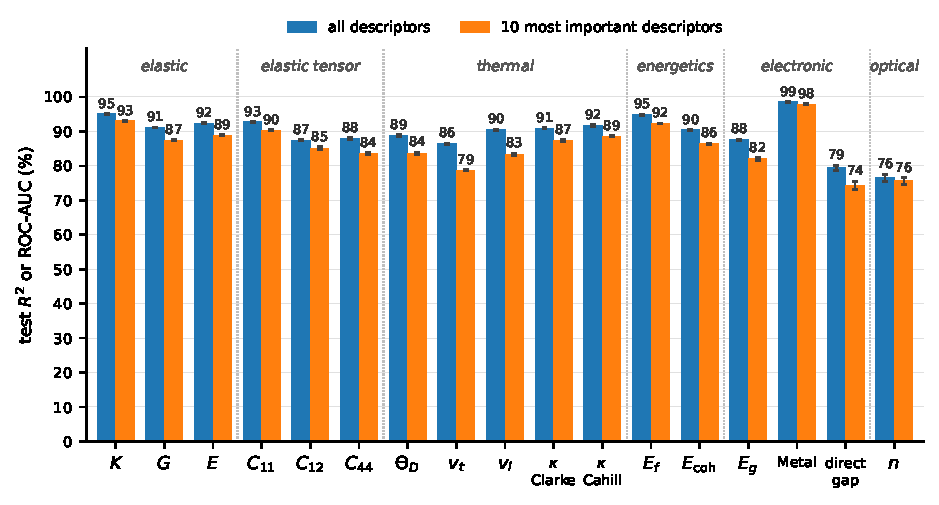
\includegraphics[width=\textwidth]{figures/fig_properties.pdf}
\caption{Test scores of LightGBM with all descriptors and with the ten most
important descriptors of each property: $R^2$, or ROC-AUC for metallicity and the
direct gap, in per cent; mean over five seeds, error bars one standard
deviation.}
\label{fig:properties}
\end{figure}

\subsection{Results and interpretation}
Table~\ref{tab:compare} compares the descriptors with models trained on the
same structures and the same split~\cite{kumar2026}: a compressed representation
of the full density grid, compositional (Magpie) features, both together, and
the graph neural networks CGCNN~\cite{xie2018} and MEGNet~\cite{chen2019}.
For this comparison our models were also trained on \rev{two properties whose
data differ from ours. The first is the energy relative to the free atoms, which
Ref.~\cite{kumar2026} computed from the DFT energies of the dataset and of the
free atoms. It is not the Materials Project cohesive energy of
Table~\ref{tab:properties}, which comes from separate calculations, and the two
differ by 0.5\,eV/atom on average. The second is the Debye temperature, which
Ref.~\cite{kumar2026} gives for fewer materials.} For the
three moduli, the descriptors alone give the highest $R^2$ of all models. For
the Debye temperature they are above the density and composition models, level
with MEGNet and behind CGCNN. For the energy relative to the free atoms they are
well above the density representation alone but below MEGNet and the models
that use the composition: this energy depends strongly on which elements are
present, which the composition describes directly.

\begin{table}[!tp]
\centering
\caption{Test $R^2$ of models trained on the same structures with the same split. All rows \rev{above the line} are from Ref.~\cite{kumar2026}; latent density: compressed representation of the full density grid. $E_{atoms}$: energy relative to the free atoms; $\Theta_D$: Debye temperature; --: not reported.}
\label{tab:compare}
\footnotesize
\begin{tabular}{@{}lccccc@{}}
\toprule
Model & $K$ & $G$ & $E$ & $E_{atoms}$ & $\Theta_D$ \\
\midrule
Latent density, CNN & 0.90 & 0.80 & 0.79 & 0.68 & 0.73 \\
Magpie, attention CNN & 0.92 & 0.85 & 0.85 & 0.88 & 0.90 \\
Latent density + Magpie, LightGBM & 0.94 & 0.87 & 0.88 & 0.96 & 0.89 \\
Latent density + Magpie, attention CNN & 0.94 & 0.85 & 0.87 & 0.88 & 0.86 \\
CGCNN & 0.93 & 0.88 & 0.89 & -- & 0.94 \\
MEGNet & 0.93 & 0.87 & 0.86 & 0.94 & 0.91 \\
\midrule
pydemi descriptors, LightGBM & 0.95 & 0.91 & 0.92 & 0.86 & 0.91 \\
\bottomrule
\end{tabular}
\end{table}

The mean interstitial density is the most important descriptor overall: it
leads for the elastic moduli and constants and for the refractive index. The
volume fraction of the NCI region plays the same role for the band gap,
metallicity and the formation energy. The thermal properties rely mainly on the
charge-distance variance, the interstitial charge fraction and the valence
Laplacian concentration, and the cohesive energy on the bond-midpoint and
interstitial densities; only the direct-gap classification has no dominant
descriptor (Supporting Information, Fig.~S5). The information is concentrated
in a few descriptors. Models trained on only the ten most important descriptors
of each property, chosen on the training set (Fig.~\ref{fig:top10};
Supporting Information, Table~S4), keep 92--99\% of the test score obtained
with all descriptors (Table~\ref{tab:properties}, Fig.~\ref{fig:properties}).
Across all properties, these lists together use 34 of the 55 descriptors, and
a few of them appear for most properties, led by the mean interstitial density,
the charge-distance variance and the negative-Laplacian volume fraction (Supporting Information, Fig.~S6). For most
properties, eight or nine of the ten are among the 44 descriptors that are
reliably computed from a predicted density (Section~\ref{sec:ml}), so the
property models should change little when the density is predicted; the next
paragraph tests this.

\begin{figure}[!t]
\centering
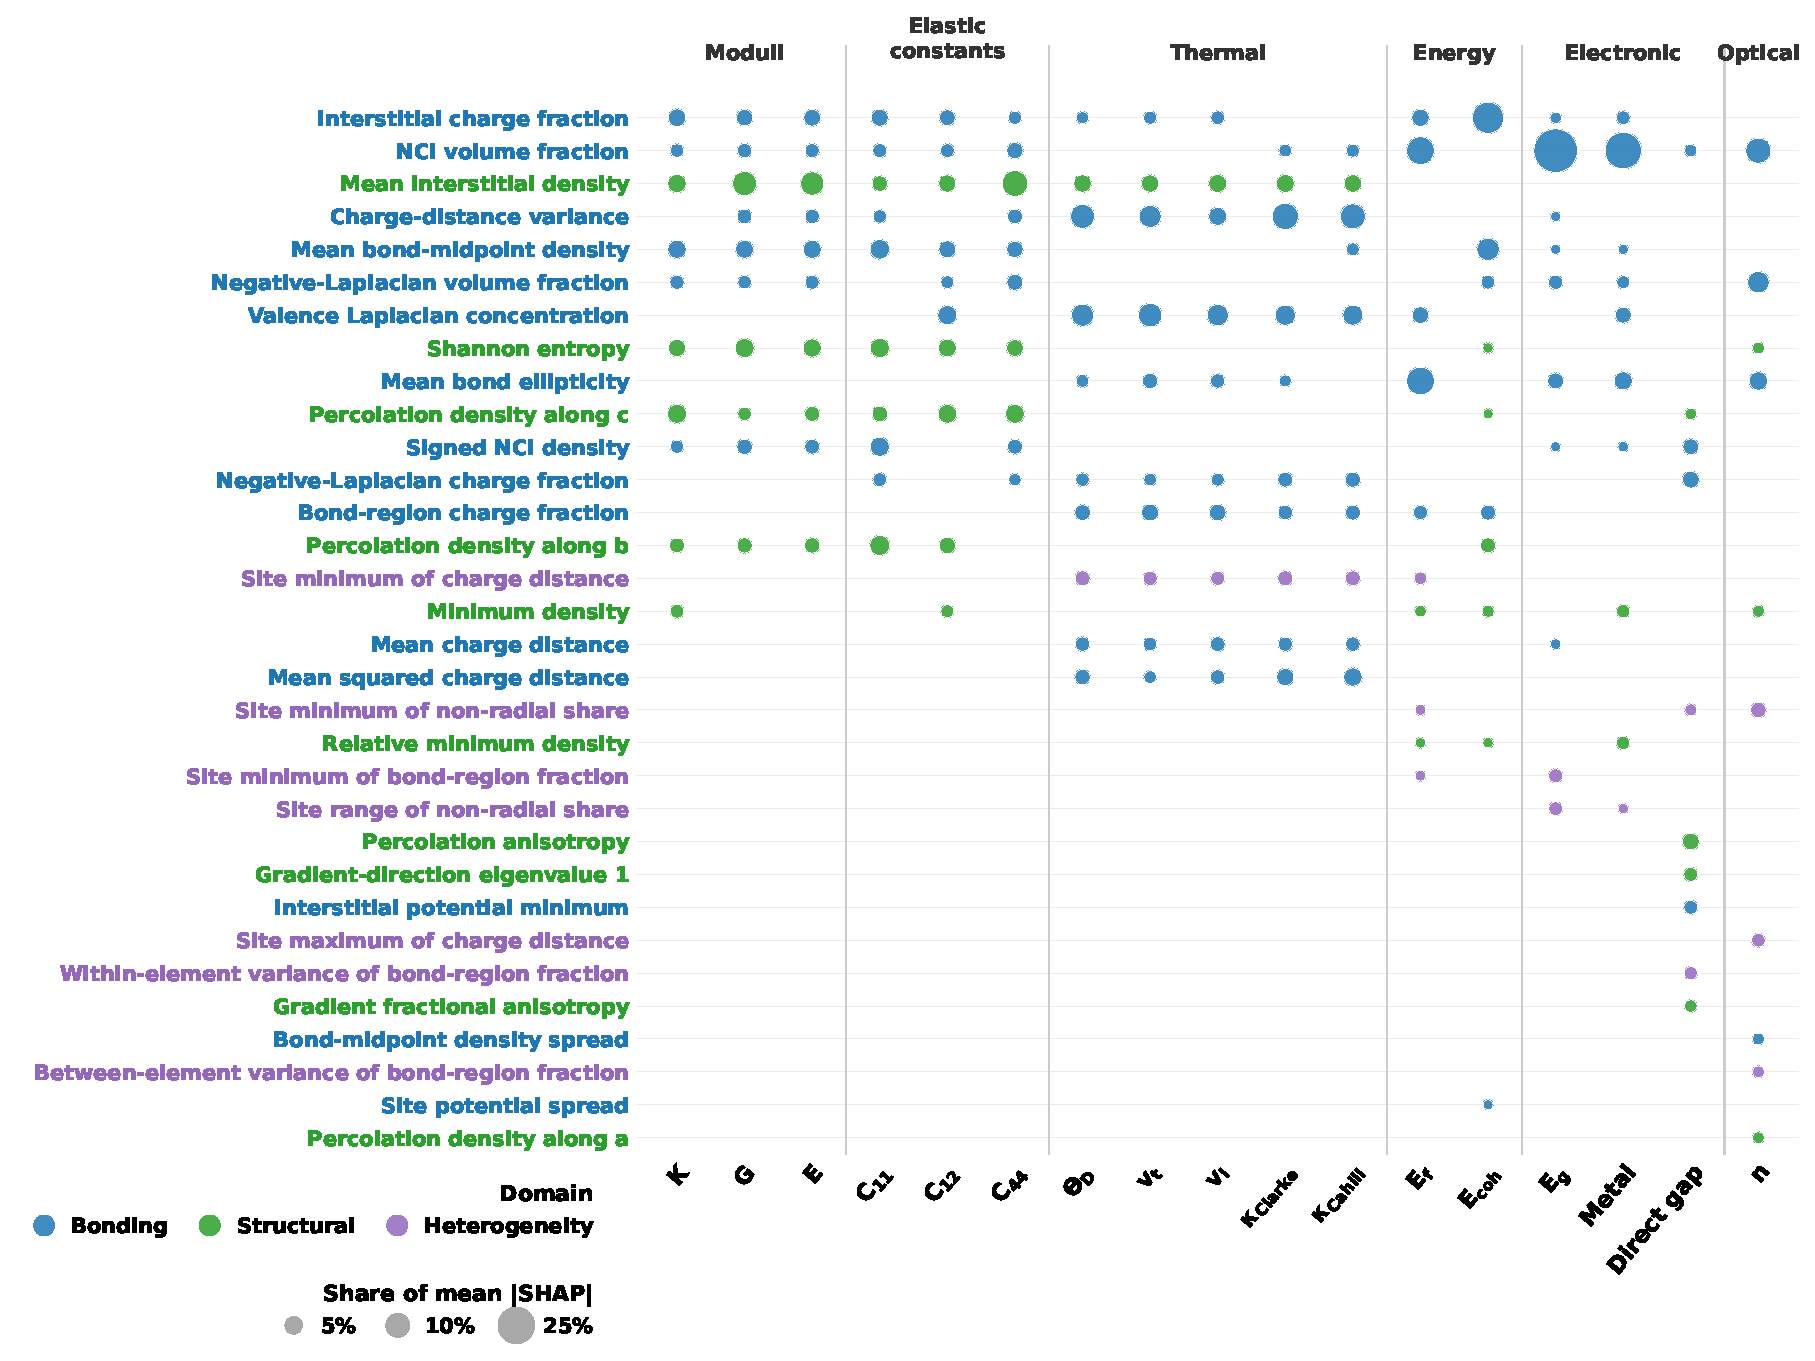
\includegraphics[width=\textwidth]{figures/fig_top10.pdf}
\caption{The ten most important descriptors of each property, ranked by their
mean absolute SHAP value in the LightGBM model with all descriptors on the training
set. A dot marks a descriptor that is among the ten of a property; its area is
the descriptor's share of the mean absolute SHAP value and its colour the
domain. Only the 34 descriptors that are among the ten for at least one property
are shown, ordered by the number of properties for which they are among the ten.}
\label{fig:top10}
\end{figure}

The descriptors can also be computed from a predicted density, and we tested
whether they still serve the property models. We trained the property models
again with the same protocol, leaving out the 605 test structures of the
density model, and evaluated them on these structures, which neither the
density model nor the property models had seen, once with the descriptors of the DFT
density and once with those of the ChargE3Net density
(Fig.~\ref{fig:mlprops}). This answers two questions: whether the two routes
give the same prediction, and how close each prediction is to the DFT value.
Because these models were trained on fewer materials (4,365 instead of 4,847)
and tested on other structures, their scores differ from those of
Table~\ref{tab:properties}, most for the shear-related properties and the
refractive index.

\begin{figure}[!t]
\centering
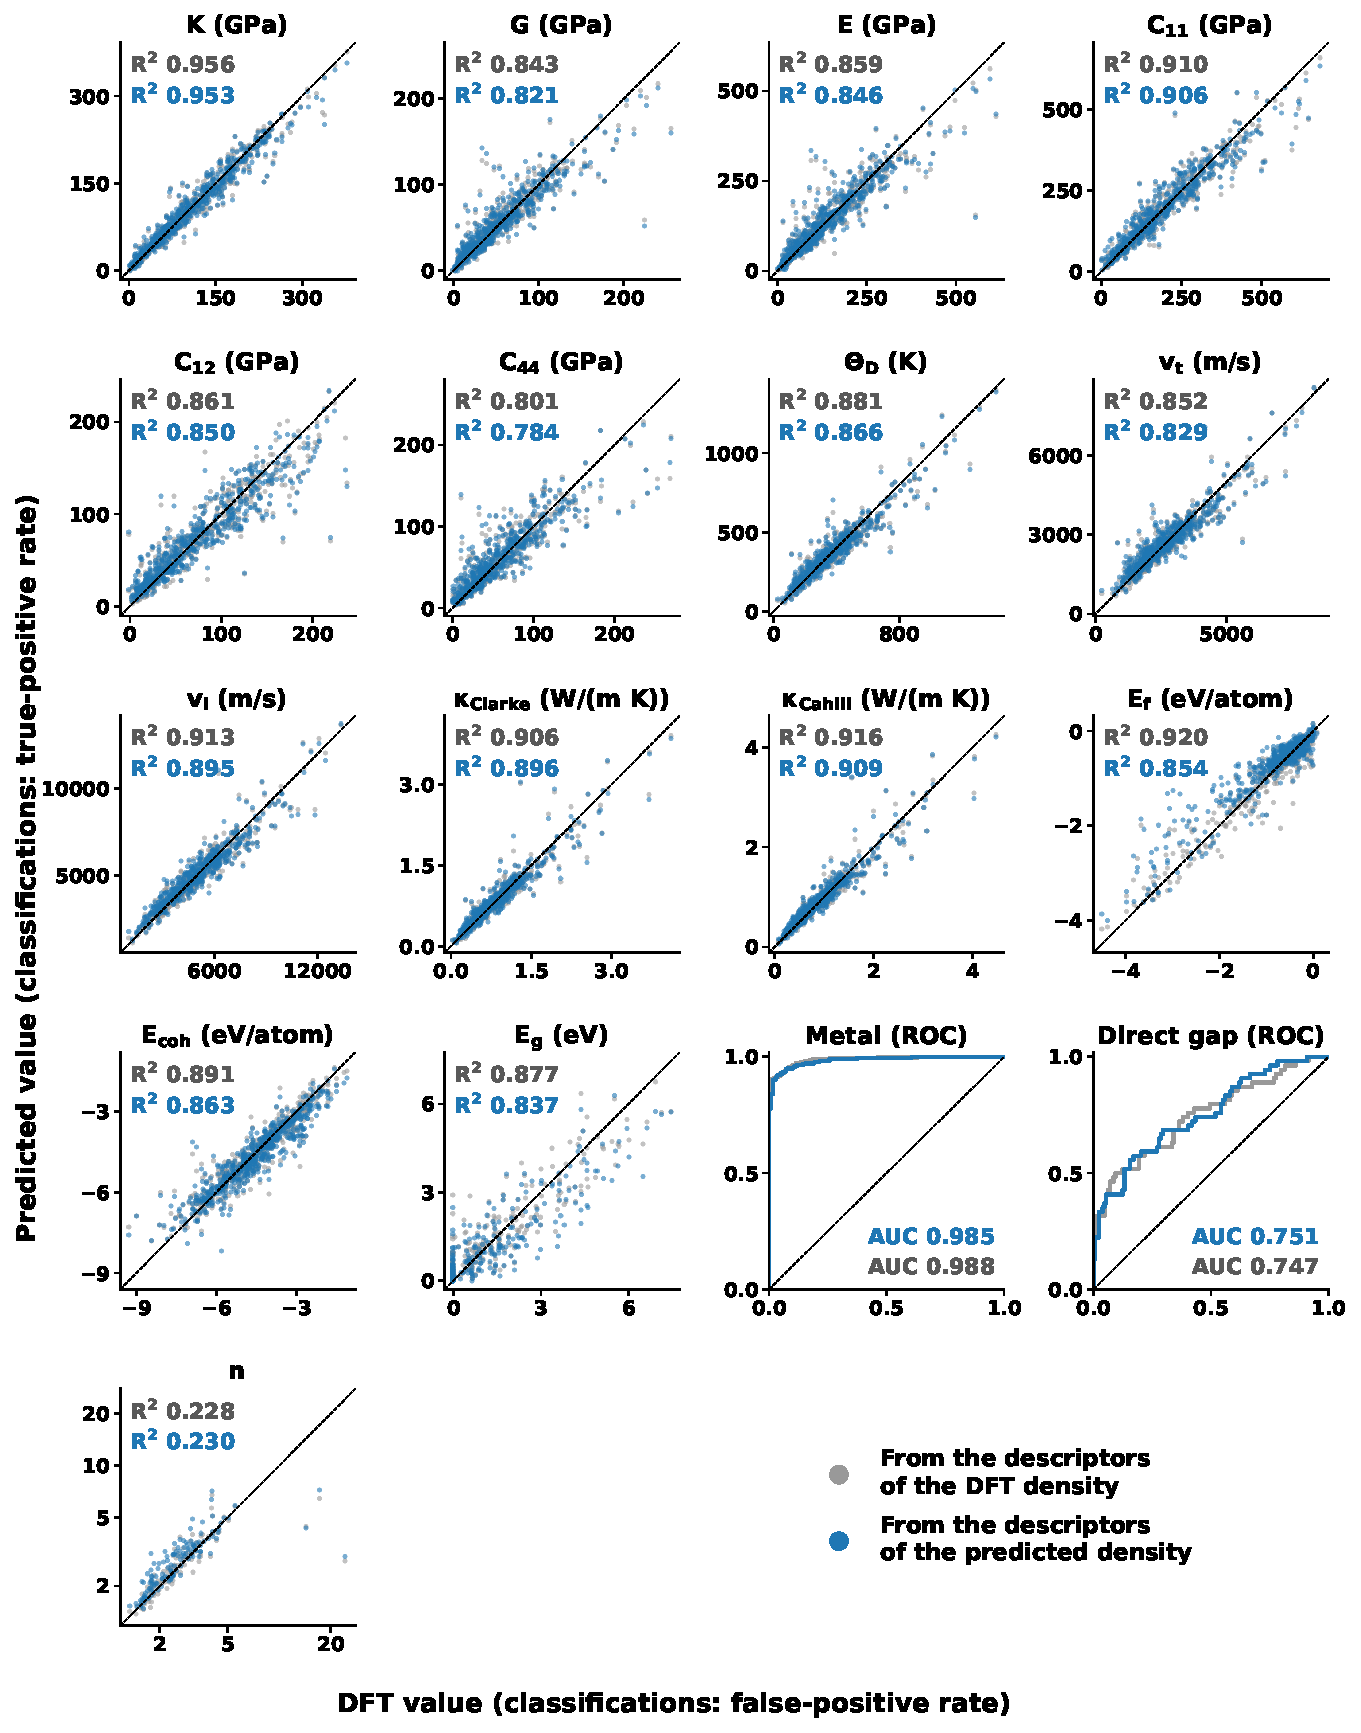
\includegraphics[width=\textwidth]{figures/fig_ml_properties.pdf}
\caption{Properties of the 605 test structures of the density model, predicted
by property models trained without them from the descriptors of the DFT density
(grey) and of the ChargE3Net density (blue), against the DFT values; for
metallicity and the direct gap, ROC curves. $R^2$ and ROC-AUC of each route
against the DFT values. The refractive index is shown on logarithmic axes.}
\label{fig:mlprops}
\end{figure}

The two routes give nearly the same predictions. For every regression property
the $R^2$ between them is at least 0.94, and they place 99.3\% of the
structures in the same metal or non-metal class. Accuracy is almost unchanged
for most properties. The bulk modulus has a test $R^2$ of 0.95 by either route,
and most other properties lose 0.01 to 0.03. The losses are largest, about 0.04, for the sound velocities, the Debye
temperature and the cohesive energy. The losses follow how much each model
relies on the 11 descriptors that transfer less well to predicted densities
(Section~\ref{sec:ml}). These descriptors carry 7\% of the importance in the
bulk-modulus model but about a fifth in the models of the sound velocities and
the Debye temperature. For the regression properties other than the refractive
index, they also cause 29 to 50\% of the difference between the two
predictions, mostly through the bond ellipticity. \rev{Whether a gap is direct is weak by either route (ROC-AUC 0.73 and 0.74). The
refractive index has an $R^2$ of only 0.17 and 0.18, but this is set by
three materials with DFT values of 14 to 24, while the other 128 lie between 1.4
and 5.5. Without these three, the $R^2$ is 0.84 from the DFT density and 0.78
from the predicted one.} All values are given in
Section~S4 and Table~S7 of the Supporting Information.

The test structures were relaxed with DFT. For a new material, the structure has
to come from elsewhere, for example from experiment or from an ML interatomic
potential, and its errors add to those measured here. Within this limit, the
descriptors and the properties of a relaxed crystal structure can be obtained
without computing its density. \rev{We did not test structures relaxed with an ML interatomic
potential. Graph networks such as CGCNN and MEGNet also predict properties from
the structure directly, with similar accuracy (Table~\ref{tab:compare}). The
route through the predicted density adds what they lack: the prediction rests on
the same 55 descriptors as for a DFT density, each with a physical meaning, so a
user can see which feature of the bonding drives it, compare the material with
those of the dataset, and check the descriptors against a DFT density once one
is computed.}

% ==========================================================================
\section{Software}
\label{sec:software}

pydemi is written in Python ($\geq$3.10) and is installed with
\texttt{pip install pydemi}. This core installation reads \texttt{CHGCAR}
files, computes the 55 descriptors of one structure or of many, and gives their
catalogue, from Python and from the command line; it needs only
NumPy~\cite{harris2020}, SciPy~\cite{virtanen2020} and
pandas~\cite{mckinney2010}. \texttt{CHGCAR} is the density format of VASP; a
density from another code, such as Quantum ESPRESSO, can be read once
it is written in this format, but the density and property models were trained
on VASP densities. Three optional extras add the rest: the graphical
interface (\texttt{pydemi[gui]}: Streamlit and Plotly, with LightGBM for the property
view), the density
model that predicts a density from a crystal structure
(\texttt{pydemi[ml]}: PyTorch~\cite{paszke2019}, e3nn~\cite{geiger2022} and
ASE~\cite{larsen2017}) and the property models (\texttt{pydemi[props]}:
LightGBM~\cite{ke2017}). A descriptor reference with the definition, formula,
physical meaning and limits of every descriptor is included and is opened from
the interface.

In Python, a density is read with \texttt{read\_chgcar} and its descriptors are
computed with \texttt{featurize}, or with \texttt{featurize\_batch} for many
files. \texttt{catalogue} returns the name, units, range and formula of every
descriptor, \texttt{ml.predict} predicts a density from a crystal structure, and
\texttt{props.predict} predicts properties from the descriptors. The command
line offers the same steps (\texttt{pydemi featurize}, \texttt{batch},
\texttt{catalogue}, \texttt{predict} and \texttt{gui}), and \texttt{pydemi
sweep} shows how the descriptors change with the shell boundaries. Batch runs
write one row per structure, with the descriptors, a flag for every value that
took its fallback and the run metadata; they continue past structures that fail
and record the error.

On our dataset, a batch run computed all descriptors of every structure without
a failure. A typical structure takes a few seconds on one processor core, and
the \rev{descriptors of the} whole dataset \rev{were computed} in well under an hour on one workstation. The
time depends mainly on the size of the density grid, not on the number of
atoms, and even the largest \texttt{CHGCAR} of the dataset needs less than a
minute and fits in the memory of an ordinary laptop (Section~S7 of the
Supporting Information).

The graphical interface (\texttt{pydemi gui}) starts a local server and opens in
the browser (Fig.~\ref{fig:gui}). An input panel on the left opens a \texttt{CHGCAR}, or a crystal structure file (CIF, POSCAR or any format ASE reads) whose density is then
predicted in the background, with its progress shown and the option to cancel.
Below it are a summary of the structure and the grid and the choice of how the cell is divided between the atoms
(Section~\ref{sec:design}). The main area has five views. The structure view shows the cell with
density slices through any lattice plane. The descriptor view lists the
descriptors by the names of Tables~\ref{tab:families} and~\ref{tab:families2}
in a searchable table, each with its formula and a figure of the
quantity it is computed from, and the plot view steps through these figures one
descriptor at a time. The property view gives the predicted properties with the
mean absolute error of each model on the test set, its test-set parity plot, its most important inputs
and, for structures of the dataset, the DFT values. The compare view (with the ML
extra) takes the \texttt{CHGCAR} shown in the input panel, predicts the density of the same structure on the same
grid, and shows the density error and the descriptors and properties from both
densities side by side. All results can be exported.

The tests of Section~\ref{sec:descriptors} check the descriptors; other tests
check the rest of the package. The reader is tested with \texttt{CHGCAR} files in
every layout VASP writes, including spin-polarized and non-collinear runs and the
older VASP~4 layout. The density model is tested by comparing its prediction for
one structure with the output of the original ChargE3Net code. The property models
are tested by comparing their predictions with those saved when the models were
trained. The interface is tested by checking that each figure is drawn from the
same numbers that give its descriptor. The tests run automatically on Linux, macOS
and Windows each time the code changes, and Section~S6 of the Supporting
Information lists all \rev{353} of them.

\begin{figure}[htbp]
\centering
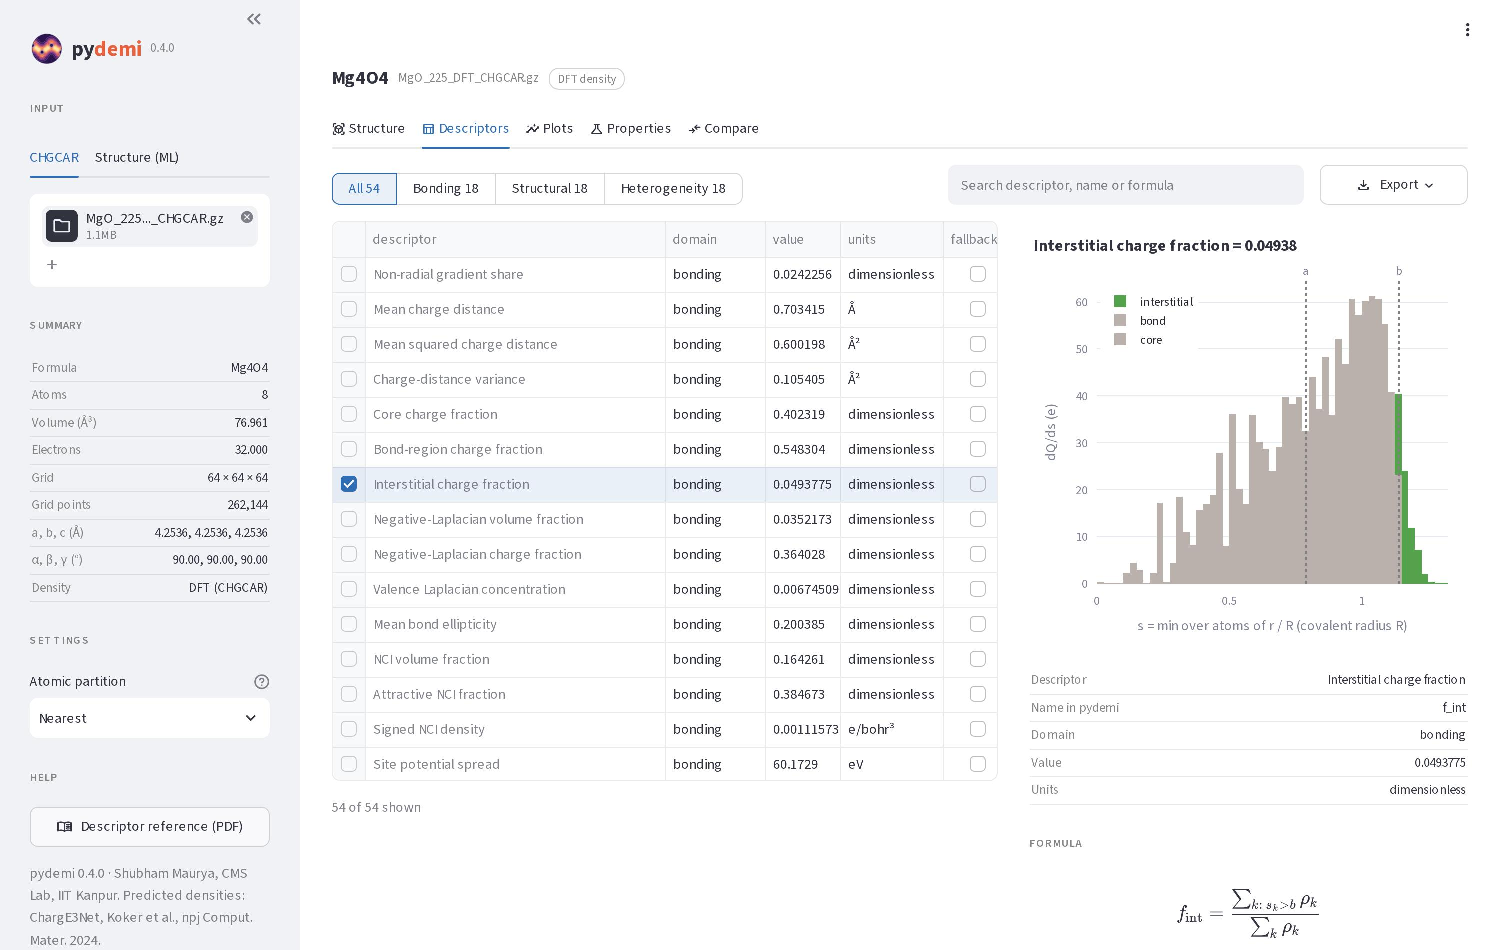
\includegraphics[width=\textwidth]{figures/fig_gui.pdf}
\caption{The graphical interface with the DFT \texttt{CHGCAR} of MgO (a
test-set structure), descriptor view: the descriptors with the interstitial
charge fraction selected, its radial charge distribution with the shell
boundaries and its formula.}
\label{fig:gui}
\end{figure}

% ==========================================================================
\section{Conclusions}
\label{sec:conclusions}
pydemi turns the one file that every VASP calculation writes, the
\texttt{CHGCAR}, into 55 descriptors, each with a short physical meaning and a
value largely set by the material rather than by the grid or the numerical
method. It computed every descriptor for every crystal of our dataset without a
failure. Automated tests compare the descriptors with exact values for model
densities and check that every descriptor stays the same when the cell is
enlarged, moved or rotated\rev{, the within-element variances of cells with one
atom per element being the only undefined case}. \rev{The descriptors do depend
on the PAW potentials of the calculation, so the property models should be applied
to densities computed with the potentials of our dataset.} It can be used
as a Python library, from the command line or through a local graphical
interface. The included ChargE3Net model gives most of the same descriptors from
a crystal structure alone. The exceptions are the counts of density maxima and
minima, quantities built from second derivatives in low-density regions, and
descriptors whose values cluster.

Used alone, the descriptors predict 17 elastic, thermal, energetic,
electronic and optical properties. SHAP values show which descriptors drive
each prediction, and ten descriptors per property are almost as good as all of
them. On \rev{DFT-relaxed} structures that neither model had seen, properties predicted from
ML-predicted densities are nearly as accurate as those from DFT densities, and
the small losses come from the descriptors that transfer less well. pydemi can
therefore predict the properties of a relaxed crystal structure without
computing its density\rev{; whether this holds for structures relaxed with an ML
interatomic potential remains to be tested}.

\section*{Code and data availability}
The source code, the tests, the descriptor reference and the scripts that train the property models are available at
\url{https://github.com/CMSLabIITK/pydemi} under the MIT license; the version described here, \rev{0.3.0}, is archived at
Zenodo (\rev{\href{https://doi.org/10.5281/zenodo.23952610}{10.5281/zenodo.23952610}; all versions: \href{https://doi.org/10.5281/zenodo.22995680}{10.5281/zenodo.22995680}}). The fine-tuned ChargE3Net checkpoint and the property models are included in the package. The ChargE3Net code included in pydemi is taken from \url{https://github.com/AIforGreatGood/charge3net} (MIT license). The
DFT dataset of charge densities was generated by members of the CMS Lab,
Department of Materials Science \& Engineering, IIT Kanpur, including the
authors, and was introduced in Ref.~\cite{kumar2026}; the data released with
that work are available at \url{https://github.com/CMSLabIITK/LatentMatFusion}.
\rev{The descriptors of all 6,059 structures and of the 605 predicted test
densities, the property targets, the test-set predictions of every model and the
PAW datasets of every calculation are deposited on Zenodo (DOI to be added).} The
DFT calculations themselves (about 180\,GB) are available from the corresponding
author upon reasonable request.

\section*{\rev{Declaration of competing interest}}
\rev{The authors declare that they have no known competing financial interests or
personal relationships that could have appeared to influence the work reported
in this paper.}

\section*{\rev{Declaration of generative AI and AI-assisted technologies in the writing process}}
\rev{During the preparation of this work the authors used Claude (Anthropic),
through Claude Code, in order to help write and test the software, prepare the
figures and tables, and edit the language of the manuscript. After using this
tool, the authors reviewed and edited the content as needed and take full
responsibility for the content of the published article.}

\section*{Acknowledgements}
We acknowledge the National Supercomputing Mission (NSM) for providing
computing resources of ``PARAM Sanganak'' at IIT Kanpur, which is implemented
by CDAC and supported by the Ministry of Electronics and Information Technology
(MeitY) and the Department of Science and Technology (DST), Government of
India. We also thank the ICME National Hub, IIT Kanpur, and CC, IIT Kanpur, for
providing an HPC facility.

\bibliographystyle{elsarticle-num}
\bibliography{references}

\end{document}

